% chapter03.tex

 %%%%%%%%%%%%%%%%%%%%%%%%%%%%%%%%%%%%%%%%%%%%%%%%%%%%%%%%%%%%%%%%%%%%%%%%%%%%%
 %                                                                           %
 %    PyMS documentation                                                     %
 %    Copyright (C) 2005-8 Vladimir Likic                                    %
 %                                                                           %
 %    The files in this directory provided under the Creative Commons        %
 %    Attribution-NonCommercial-NoDerivs 2.1 Australia license               %
 %    http://creativecommons.org/licenses/by-nc-nd/2.1/au/                   %
 %    See the file license.txt                                               %
 %                                                                           %
 %%%%%%%%%%%%%%%%%%%%%%%%%%%%%%%%%%%%%%%%%%%%%%%%%%%%%%%%%%%%%%%%%%%%%%%%%%%%%

\chapter{GC-MS Intensity Matrix}



\section{Converting Raw GC-MS data to an Intensity Matrix}

\noindent
[ {\em This example is in pyms-test/02} ]


\section{Ion Chromatogram}

\section{Mass Spectrum}

\section{Saving data}


% %%%%%%%%%%%%%%%%%%%%%%%%%%%%%%%%%%%%%%%%%%%%%%%%%%%%%%%%%%%%%%%%%
% \chapter{Intensity Matrix}
% Each scan only
% contains information about the mass/charge and intensity at intensity peaks in
% the scan. This means that consecutive scans do not necessarily contain the
%same
% mass/charge values. For data processing, it is often necessary to convert the
% data to a matrix with a set number of mass/charge values and number of scans.
% This means some mechanism for converting mass/charge values to a set of fixed
% values is required. In PyMS there are functions to explicitly handle the
% conversion of mass/charge values to consistent values across all scans.
%
% The general scheme for converting mass/charge values is to bin intensity
% values
% based on the interval the corresponding mass/charge values belongs to. The
% general procedure is
% as follows:
% \begin{itemize}
%     \item for a given bin size
%     \item determine the maximum and minimum mass/charge values in entire data
%set.
%     \item calculate the number of bins in the total mass/charge range.
%     \item centre the first bin at the minimum mass/charge value.
%     \item sum intensities corresponding to all mass/charge values that are in
%a
% given bin.
% \end{itemize}
%
% A specific function to round mass/charge values is also available. The
% process is that all intensity values for a mass/charge values that fall within
%a
% unit width about each given integer value are added together. In PyMS, a
% mass/charge is considered to belong to a bin when it is equal to or greater
% than half the bin width from the centre of the bin, and less than half the bin
% width from the centre of the bin.
% %That is, a mass/charge, $m$ is considered to belong to a bin when $c-w/2\le
% %m\lt c+w/2$, where $c$ is the centre of the bin, and $w$ is the width of the
% %bin.
%
% Figure~\ref{fig:binning} illustrates the process of assigning bins to the
% mass/charge axis and summing all intensities in a given bin. The result is a
% new mass/charge axis with mass/charge values corresponding to the centre of
% each bin.
%
% \begin{figure}[htp]
% \begin{center}
% \includegraphics{graphics/binning/binning.eps}
% \caption{Mass/charge intensity values are added to bins based on a pre-set bin
% size and the minimum mass/charge value of all the scan data. All intensities
%in
% a given bin width (top) are added and given a mass/charge value of the centre
% of the bin (bottom). For integer binning, each bin has a width of one and is
% centred at integer values.}
% \label{fig:binning}
% \end{center}
% \end{figure}
%
% %%%%%%%%%%%%%%%%%%%%%%%%%%%%%%%%%%%%%%%%%%%%%%%%%%%
% \noindent
% An IonChromatogram object is a one dimensional vector containing
% mass intensities as a function of retention time. This can can be either
% m/z channel intensities (for example, ion chromatograms at m/z = 65),
% or cumulative intensities over all measured m/z (TIC).
%
% An ion chromatogram object has a method {\tt is\_tic()} which returns
% True is the ion chromatogram is TIC, False otherwise:
%
% \begin{verbatim}
% >>> print "'tic' is a TIC:", tic.is_tic()
% 'tic' is a TIC: True
% >>> print "'ic' is a TIC:",ic.is_tic()
% 'ic' is a TIC: False
% \end{verbatim}
%
% \subsection{Writing data to a file}
%
% The method {\tt write()} of IonChromatogram object allows one to save
% the ion chromatogram object to a file:
%
% \begin{verbatim}
% >>> tic.write("output/tic.dat", minutes=True)
% >>> ic.write("output/ic.dat", minutes=True)
% \end{verbatim}
%
% \noindent
% The flag minutes=True indicates that retention time will be saved in minutes.
% The ion chromatogram object saved with with the {\tt write{}} method is a
% plain ASCII file which contains a pair of (retention time, intensity) per
% line:
%
% \begin{verbatim}
% $ head tic.dat
%   5.0944      745997.0000
%   5.1002      726566.0000
%   5.1059      717704.0000
%   5.1116      684214.0000
%   5.1173      701866.0000
%   5.1230      893306.0000
%   5.1287     1278099.0000
%   5.1345     1290984.0000
%   5.1402      925558.0000
%   5.1459      644122.0000
% \end{verbatim}
%
% \noindent
% Figure \ref{fig:tic-plot} shows the plot of the file 'tic.dat' produced with
%the
% program Gnuplot. The Gnuplot script used to produce this plot is provided
% as pyms-test/01/output/plot.gnu.
%
% \begin{figure}[htp]
% \begin{center}
% %x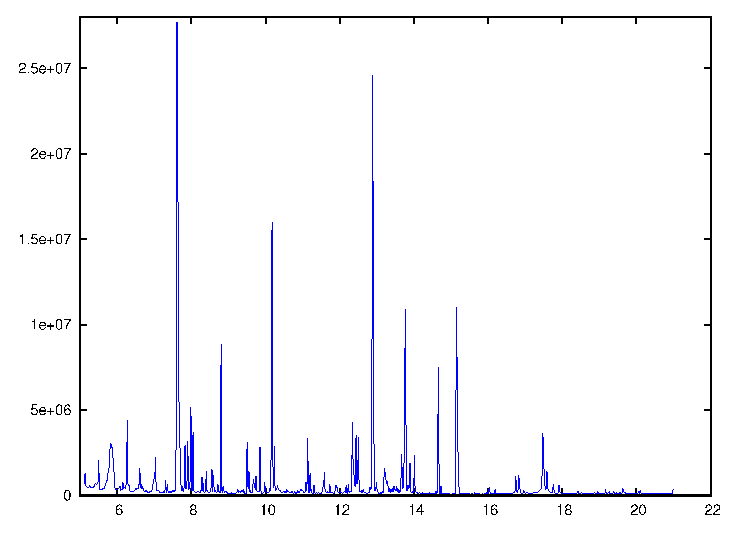
\includegraphics{graphics/pyms-test/tic.eps}
% \caption{The Gnuplot plot of the file 'tic.dat'}
% \label{fig:tic-plot}
% \end{center}
% \end{figure}

jcamp_file = "/x/PyMS/data/gc01_0812_066.jdx"
data = JCAMP_reader(jcamp_file)

# IntensityMatrix
# must build intensity matrix before accessing any intensity matrix methods.

# default, float masses with interval (bin size) of one from min mass
print "default intensity matrix, bin size = 1"
im = build_intensity_matrix(data)

print "size of intensity matrix (#scans, #bins):", im.get_size()

masses = im.get_mass_list()

print "start mass:", min(masses)
print "end mass:", max(masses)

index = im.get_index_of_mass(73.3)
print "the index of the nearest mass to 73.3m/z is:", index
print "the nearest mass to 73.3m/z is:", masses[index]
print

# bin size of 0.5, eg. for double charge ions
print "intensity matrix, bin size = 0.5"
im = build_intensity_matrix(data, 0.5)

print "size of intensity matrix (#scans, #bins):", im.get_size()

masses = im.get_mass_list()

print "start mass:", min(masses)
print "end mass:", max(masses)

index = im.get_index_of_mass(73.3)
print "the index of the nearest mass to 73.3m/z is:", index
print "the nearest mass to 73.3m/z is:", masses[index]
print

# integer intensity matrix, integer masses, in one unit steps
print "intensity matrix with integer mass and bin size = 1"
im = build_intensity_matrix_i(data)

print "size of intensity matrix (#scans, #bins):", im.get_size()

masses = im.get_mass_list()

print "start mass:", min(masses)
print "end mass:", max(masses)

index = im.get_index_of_mass(73.3)
print "the index of the nearest mass to 73.3m/z is:", index
print "the nearest mass to 73.3m/z is:", masses[index]
print

# TIC and SIC

# TIC from raw data
tic = data.get_tic()
# save TIC to a file
tic.write("output/tic.dat",minutes=True)

# get the first ion chromatogram of the IntensityMatrix
ic = im.get_ic_at_index(0)
ic.write("output/ic_index_1.dat",minutes=True)
# get the ion chromatogram for m/z = 73
ic = im.get_ic_at_mass(73)
ic.write("output/ic_mass_73.dat",minutes=True)

# some tests on ion chromatogram objects
print "'tic' is a TIC:", tic.is_tic()
print "'ic' is a TIC:", ic.is_tic()
print

# Data saving

# save the intensity matrix values to a file
mat = im.get_matrix_list()
print "saving intensity matrix intensity values..."
save_data("output/im.dat", mat)

# Export the entire IntensityMatrix as CSV. This will create
# data.im.csv, data.mz.csv, and data.rt.csv where
# these are the intensity matrix, retention time
# vector, and m/z vector in the CSV format
print "exporting intensity matrix data..."
export_csv("output/data", im)

# Export the entire IntensityMatrix as LECO CSV. This is
# useful for import into AnalyzerPro
print "exporting intensity matrix data to LECO CSV format..."
export_leco_csv("output/data_leco.csv", im)
